\documentclass[border=1mm]{standalone}

\usepackage{pgfplots}
\pgfplotsset{compat=1.13}
%\usepackage{tikz,tikz-3dplot} %Para fazer desenhos
\usetikzlibrary{shapes.multipart,shapes.geometric,calc,angles,positioning,intersections,quotes,decorations,babel,patterns,fit}
\usepackage{tkz-euclide}
\usetkzobj{all}

\begin{document}
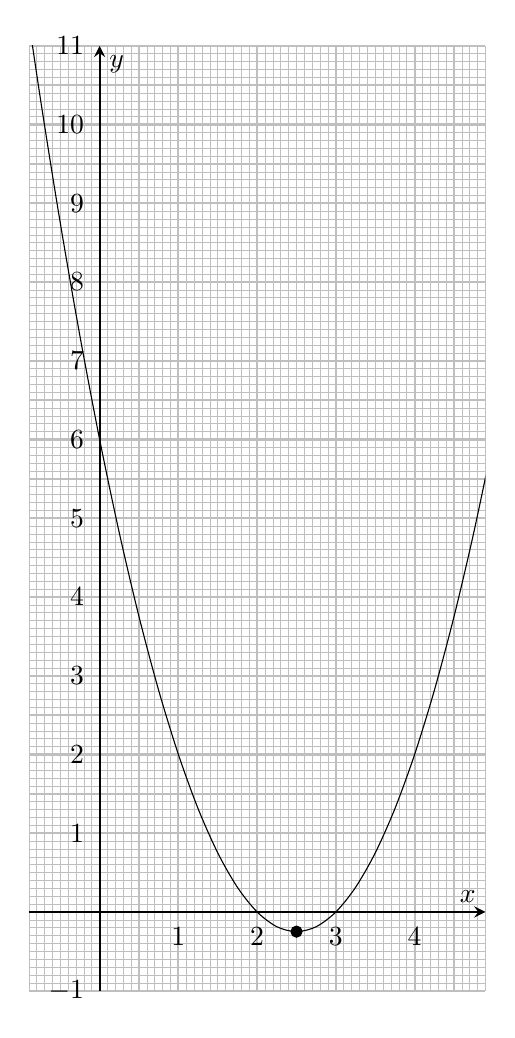
\begin{tikzpicture}[%
    % style for middle grid
    middle grid style/.style={lightgray,line width=0.5pt}
]
\pgfplotsset{%
    % enable layer, needed to draw middle grid below axis
    set layers=standard,
    % disable ticks
    every major tick/.style={draw=none},
    every minor tick/.style={draw=none},
}
\begin{axis}    [
axis lines = {center},
% set fixed scale to get mm grid
% note: this is for the major grid
x=1cm,
y=1cm,
ylabel = {$y$},
xlabel = {$x$},
ytick distance = 1,
xtick distance = 1,
% number of minor ticks between 2 major ticks
minor x tick num=9,
minor y tick num=9,
ymin=-1,
ymax=11,
xmin=-0.9,
xmax=4.9,
major grid style={lightgray,thick},
minor grid style={lightgray,very thin},
grid=both,
% optional stuff
% change axis line width
axis line style={thick},
% make tick labels cover the grid
%ticklabel style={inner sep=1pt,fill=white},
]

% draw middle grid
\begin{pgfonlayer}{axis grid}
% works only for x=y=1cm with plots
%\draw[middle grid style,step=0.5cm]
%    (axis cs:\pgfkeysvalueof{/pgfplots/xmin},\pgfkeysvalueof{/pgfplots/ymin}) grid
%    (axis cs:\pgfkeysvalueof{/pgfplots/xmax},\pgfkeysvalueof{/pgfplots/ymax});
% to be used for graph paper with no plots (and if x != y)
%               v-- first, second and last x-positions for middle grid
\foreach \x in {-0.5,0.5,...,4.5}{
    % \edef-trick, see manual page 541
    \edef\temp{\noexpand\draw[middle grid style]
        (axis cs:\x,\pgfkeysvalueof{/pgfplots/ymin}) --
        (axis cs:\x,\pgfkeysvalueof{/pgfplots/ymax});}
    \temp
}
%               v-- first, second and last y-positions for middle grid
\foreach \y in {-0.5,0.5,...,10.5}{
    \edef\temp{\noexpand\draw[middle grid style]
        (axis cs:\pgfkeysvalueof{/pgfplots/xmin},\y) --
        (axis cs:\pgfkeysvalueof{/pgfplots/xmax},\y);}
    \temp
}
\end{pgfonlayer}

\addplot    [
mark = none, domain= -1:5, smooth %samples at = {-1,0,1,2,3,4,5}
]
{x^2 -5*x + 6};

\addplot    [
mark=*
]
coordinates {(2.5,-0.25)};
\end{axis}
\end{tikzpicture}
\end{document}
